\documentclass[11pt, a4paper]{article}
\usepackage{pdfpages}
\usepackage{parallel}
\usepackage[T2A]{fontenc}
\usepackage{ucs}
\usepackage[utf8x]{inputenc}
\usepackage[polish,english,russian]{babel}
\usepackage{hyperref}
\usepackage{rotating}
\usepackage[inner=2cm,top=1.8cm,outer=2cm,bottom=2.3cm,nohead]{geometry}
\usepackage{listings}
\usepackage{graphicx}
\usepackage{wrapfig}
\usepackage{longtable}
\usepackage{indentfirst}
\usepackage{array}
\usepackage{tikzsymbols}
\usepackage{soul}
\usepackage[ruled,vlined]{algorithm2e}
%\counterwithout{figure}{section} 

\usepackage{url}
\makeatletter
\g@addto@macro{\UrlBreaks}{\UrlOrds}
\makeatother

\newcolumntype{P}[1]{>{\raggedright\arraybackslash}p{#1}}
\frenchspacing
\usepackage{fixltx2e} %text sub- and superscripts
\usepackage{icomma} % коскі ў матэматычным рэжыме
\PreloadUnicodePage{4}

\newcommand{\longpage}{\enlargethispage{\baselineskip}}
\newcommand{\shortpage}{\enlargethispage{-\baselineskip}}

\def\switchlang#1{\expandafter\csname switchlang#1\endcsname}
\def\switchlangbe{
\let\saverefname=\refname%
\def\refname{Літаратура}%
\def\figurename{Іл.}%
}
\def\switchlangen{
\let\saverefname=\refname%
\def\refname{References}%
\def\figurename{Fig.}%
}
\def\switchlangru{
\let\saverefname=\refname%
\let\savefigurename=\figurename%
\def\refname{Литература}%
\def\figurename{Рис.}%
}

\hyphenation{admi-ni-stra-tive}
\hyphenation{ex-pe-ri-ence}
\hyphenation{fle-xi-bi-li-ty}
\hyphenation{Py-thon}
\hyphenation{ma-the-ma-ti-cal}
\hyphenation{re-ported}
\hyphenation{imp-le-menta-tions}
\hyphenation{pro-vides}
\hyphenation{en-gi-neering}
\hyphenation{com-pa-ti-bi-li-ty}
\hyphenation{im-pos-sible}
\hyphenation{desk-top}
\hyphenation{elec-tro-nic}
\hyphenation{com-pa-ny}
\hyphenation{de-ve-lop-ment}
\hyphenation{de-ve-loping}
\hyphenation{de-ve-lop}
\hyphenation{da-ta-ba-se}
\hyphenation{plat-forms}
\hyphenation{or-ga-ni-za-tion}
\hyphenation{pro-gramming}
\hyphenation{in-stru-ments}
\hyphenation{Li-nux}
\hyphenation{sour-ce}
\hyphenation{en-vi-ron-ment}
\hyphenation{Te-le-pathy}
\hyphenation{Li-nux-ov-ka}
\hyphenation{Open-BSD}
\hyphenation{Free-BSD}
\hyphenation{men-ti-on-ed}
\hyphenation{app-li-ca-tion}

\def\progref!#1!{\texttt{#1}}
\renewcommand{\arraystretch}{2} %Іначай формулы ў матрыцы зліпаюцца з лініямі
\usepackage{array}

\def\interview #1 (#2), #3, #4, #5\par{

\section[#1, #3, #4]{#1 -- #3, #4}
\def\qname{LVEE}
\def\aname{#1}
\def\q ##1\par{{\noindent \bf \qname: ##1 }\par}
\def\a{{\noindent \bf \aname: } \def\qname{L}\def\aname{#2}}
}

\def\interview* #1 (#2), #3, #4, #5\par{

\section*{#1\\{\small\rm #3, #4. #5}}
\ifx\ParallelWhichBox\undefined%
    \addcontentsline{toc}{section}{#1, #3, #4}%
\else%
\ifnum\ParallelWhichBox=0%
    \addcontentsline{toc}{section}{#1, #3, #4}%
\fi\fi%

\def\qname{LVEE}
\def\aname{#1}
\def\q ##1\par{{\noindent \bf \qname: ##1 }\par}
\def\a{{\noindent \bf \aname: } \def\qname{L}\def\aname{#2}}
}

\newcommand{\interviewfooter}[1]{
\vskip 1em
\noindent \textit{#1}
}


\begin{document}

\title{1996 "--- Hi-Bon Optical laser mouse LMOX-2}
\date{}
\maketitle

The Hi-Bon Optical laser mouse LMOX-2 (figure \ref{fig:OpticalLaserMousePic}) was produced in South Korea and was, along with the Q500 mouse, one of two unusual optical mice developed in 1996 by iO TEK that use light fibers. The resolution of this mouse is 450 dpi. The box mentions as a revolutionary feature the absence of a ball and, accordingly, the absence of the need for cleaning.

\begin{figure}[h]
    \centering
    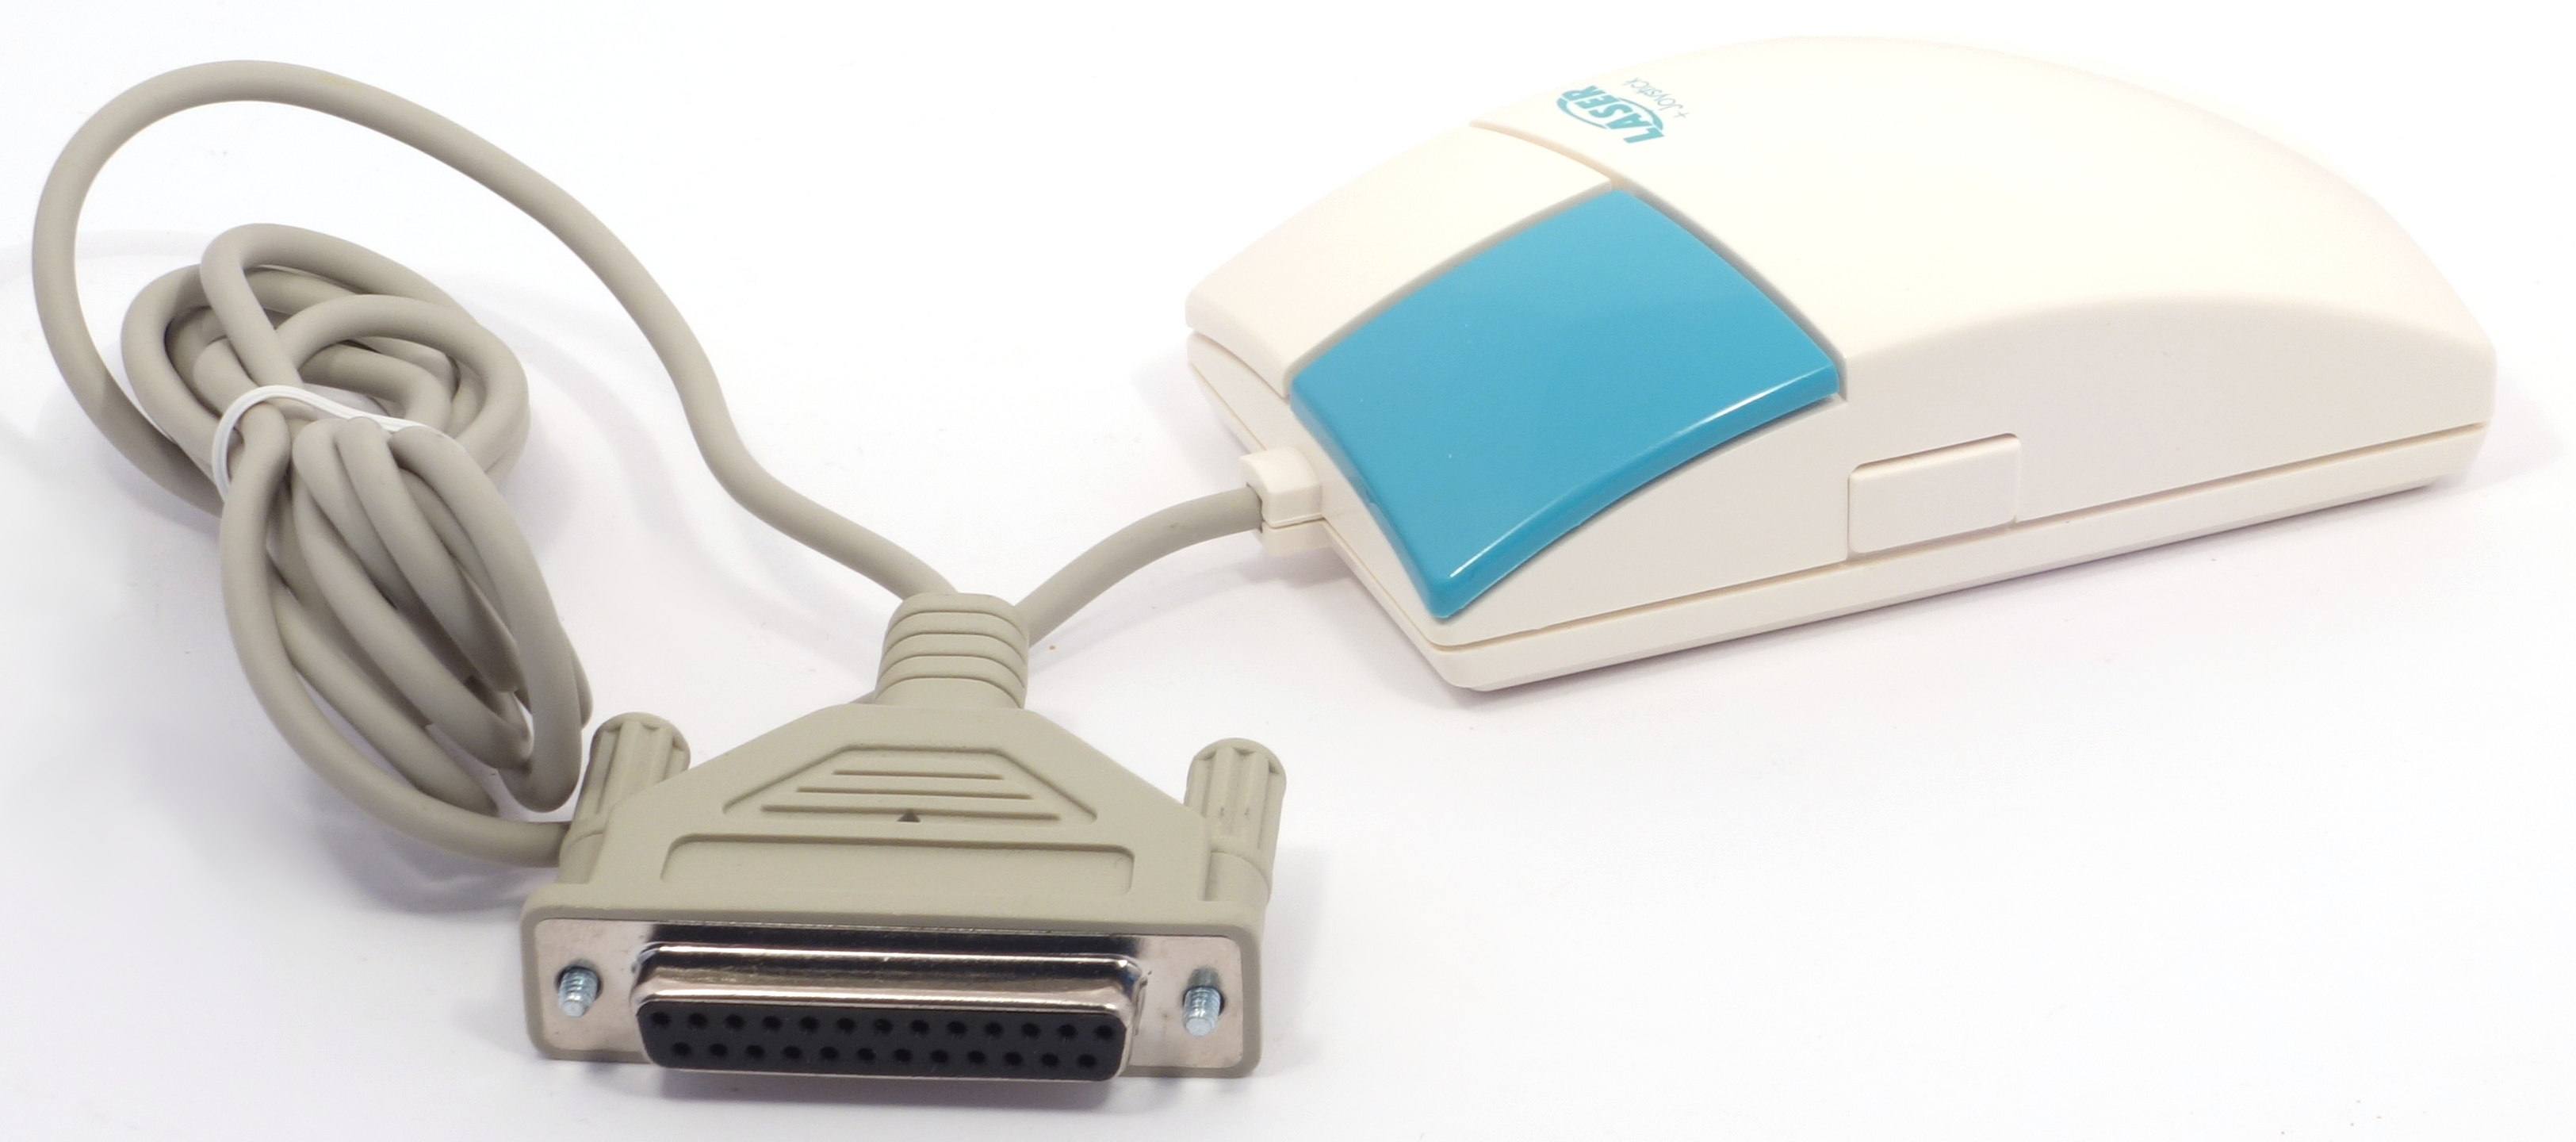
\includegraphics[scale=0.4]{1996_hi-bon_laser_mouse/pic_30.jpg}
    \caption{Hi-Bon Optical laser mouse}
    \label{fig:OpticalLaserMousePic}
\end{figure}

As with the vast majority of early optical mice, this mouse requires a reflective mesh pad (figure \ref{fig:OpticalLaserMousePad}). Unlike Mouse Systems' metal mats, this one has a white IR reflective surface with black dots applied to it, which are less reflective in the IR range. The pad has a small size, which, however, is compensated by the high resolution of the mouse.и.

\begin{figure}[h]
    \centering
    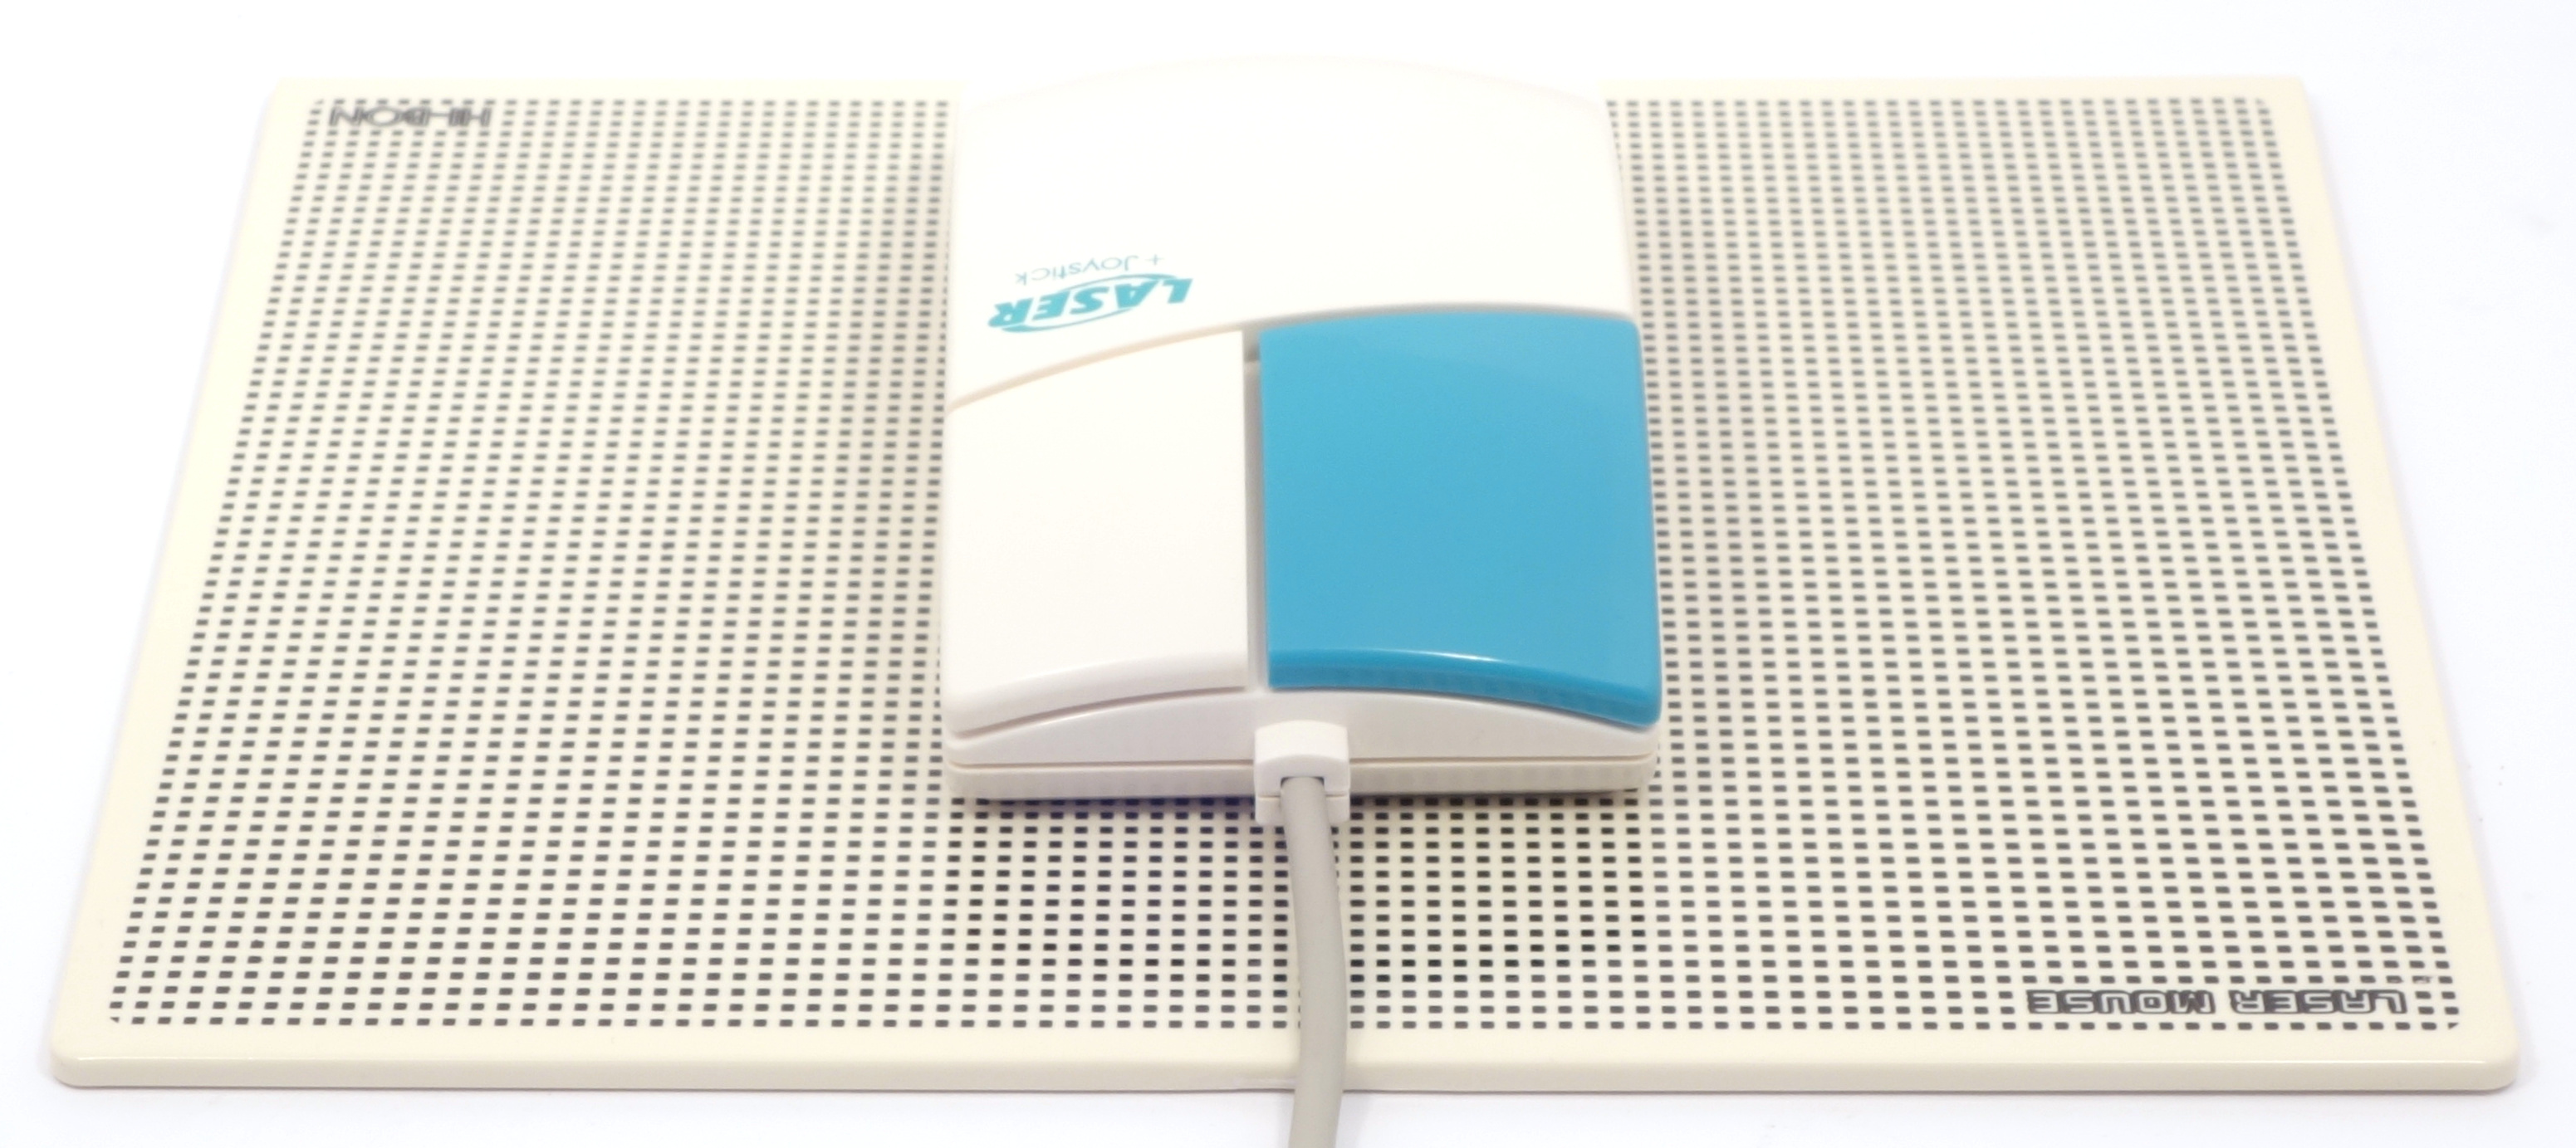
\includegraphics[scale=0.4]{1996_hi-bon_laser_mouse/pic2_30.jpg}
    \caption{Hi-Bon Optical laser mouse на комплектном коврике}
    \label{fig:OpticalLaserMousePad}
\end{figure}

The mouse has a minimalistic design and two buttons, one of which differs in color (in the second half of the 90s, this was more of a design decision than an attempt to clearly show the user where the main mouse button is). From the bottom side, two LEDs and outputs of 16 light fibers are visible (figure \ref{fig:OpticalLaserMouseTopBottom}).

\begin{figure}[h]
    \centering
    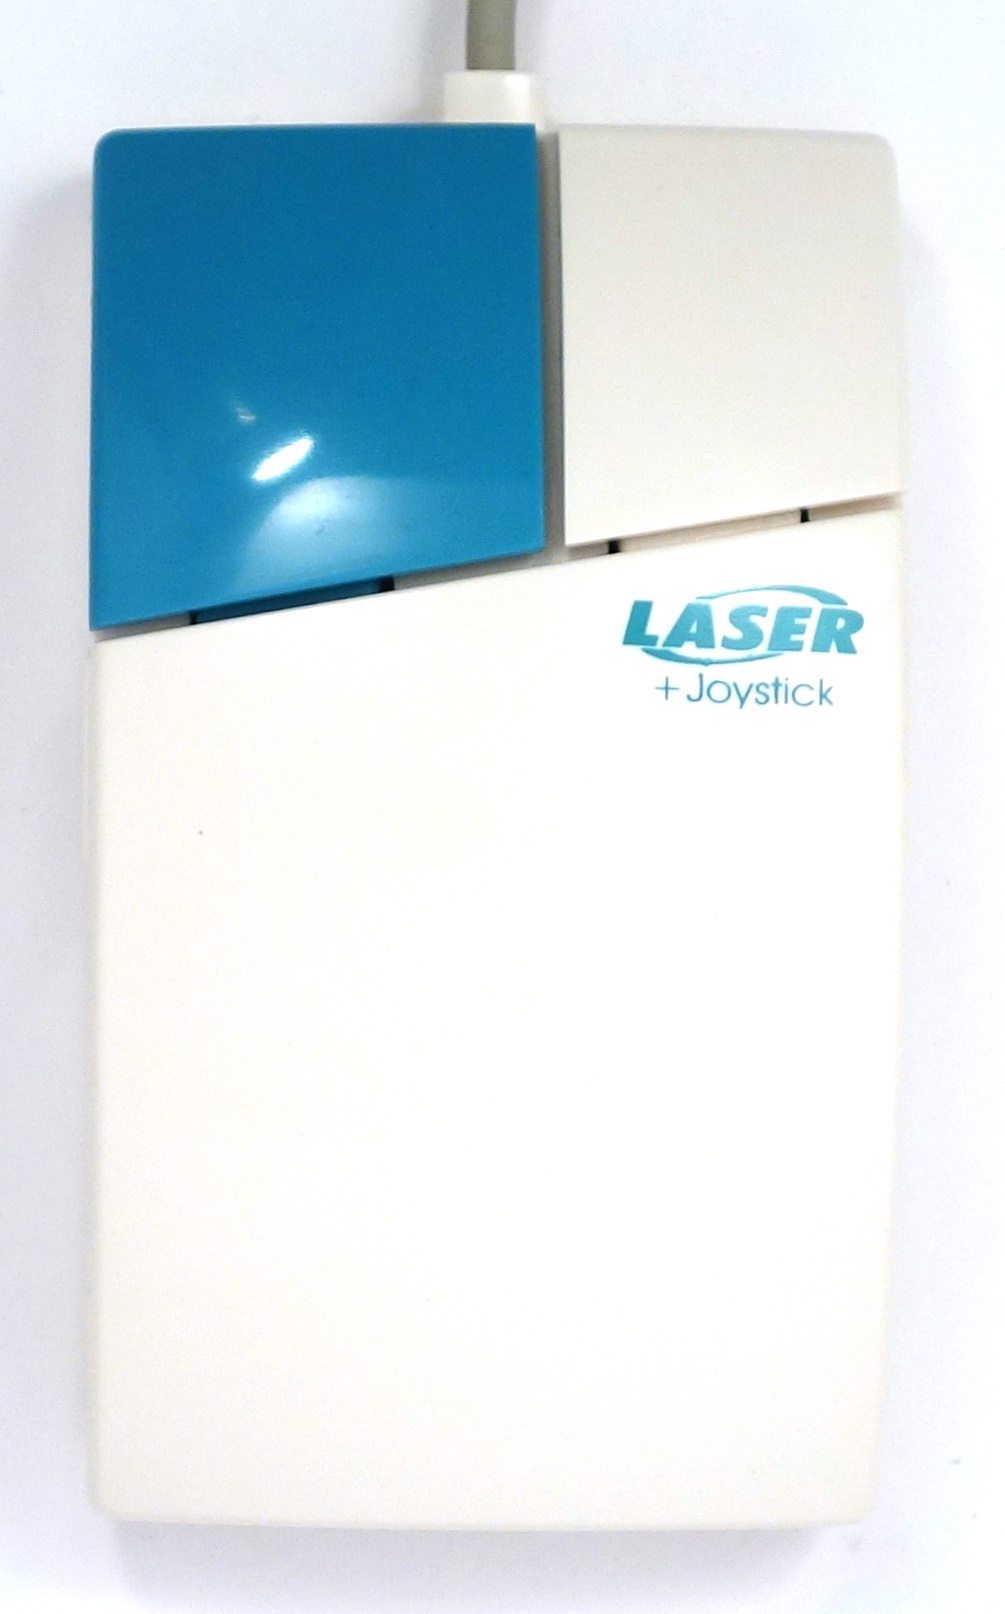
\includegraphics[scale=0.4]{1996_hi-bon_laser_mouse/top_60.jpg}
    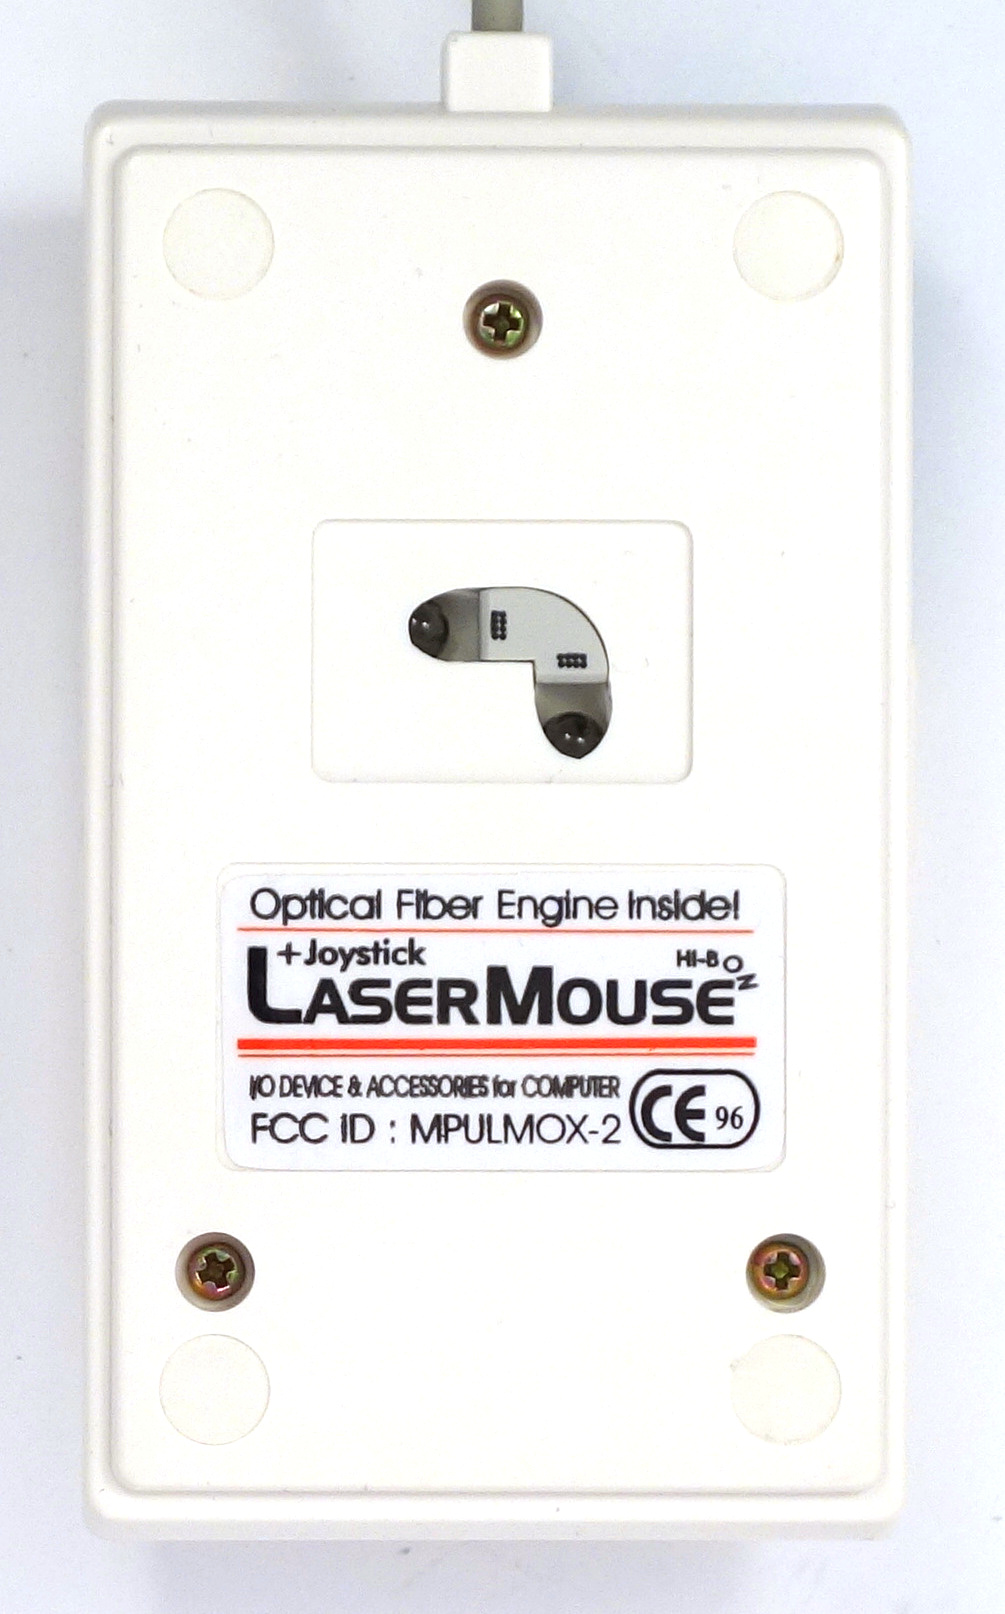
\includegraphics[scale=0.4]{1996_hi-bon_laser_mouse/bottom_60.jpg}
    \caption{Hi-Bon Optical laser mouse, top and bottom views}
    \label{fig:OpticalLaserMouseTopBottom}
\end{figure}

This mouse is a two-button device of typical size and shape (figure \ref{fig:OpticalLaserMouseSize}).

\begin{figure}[h]
    \centering
    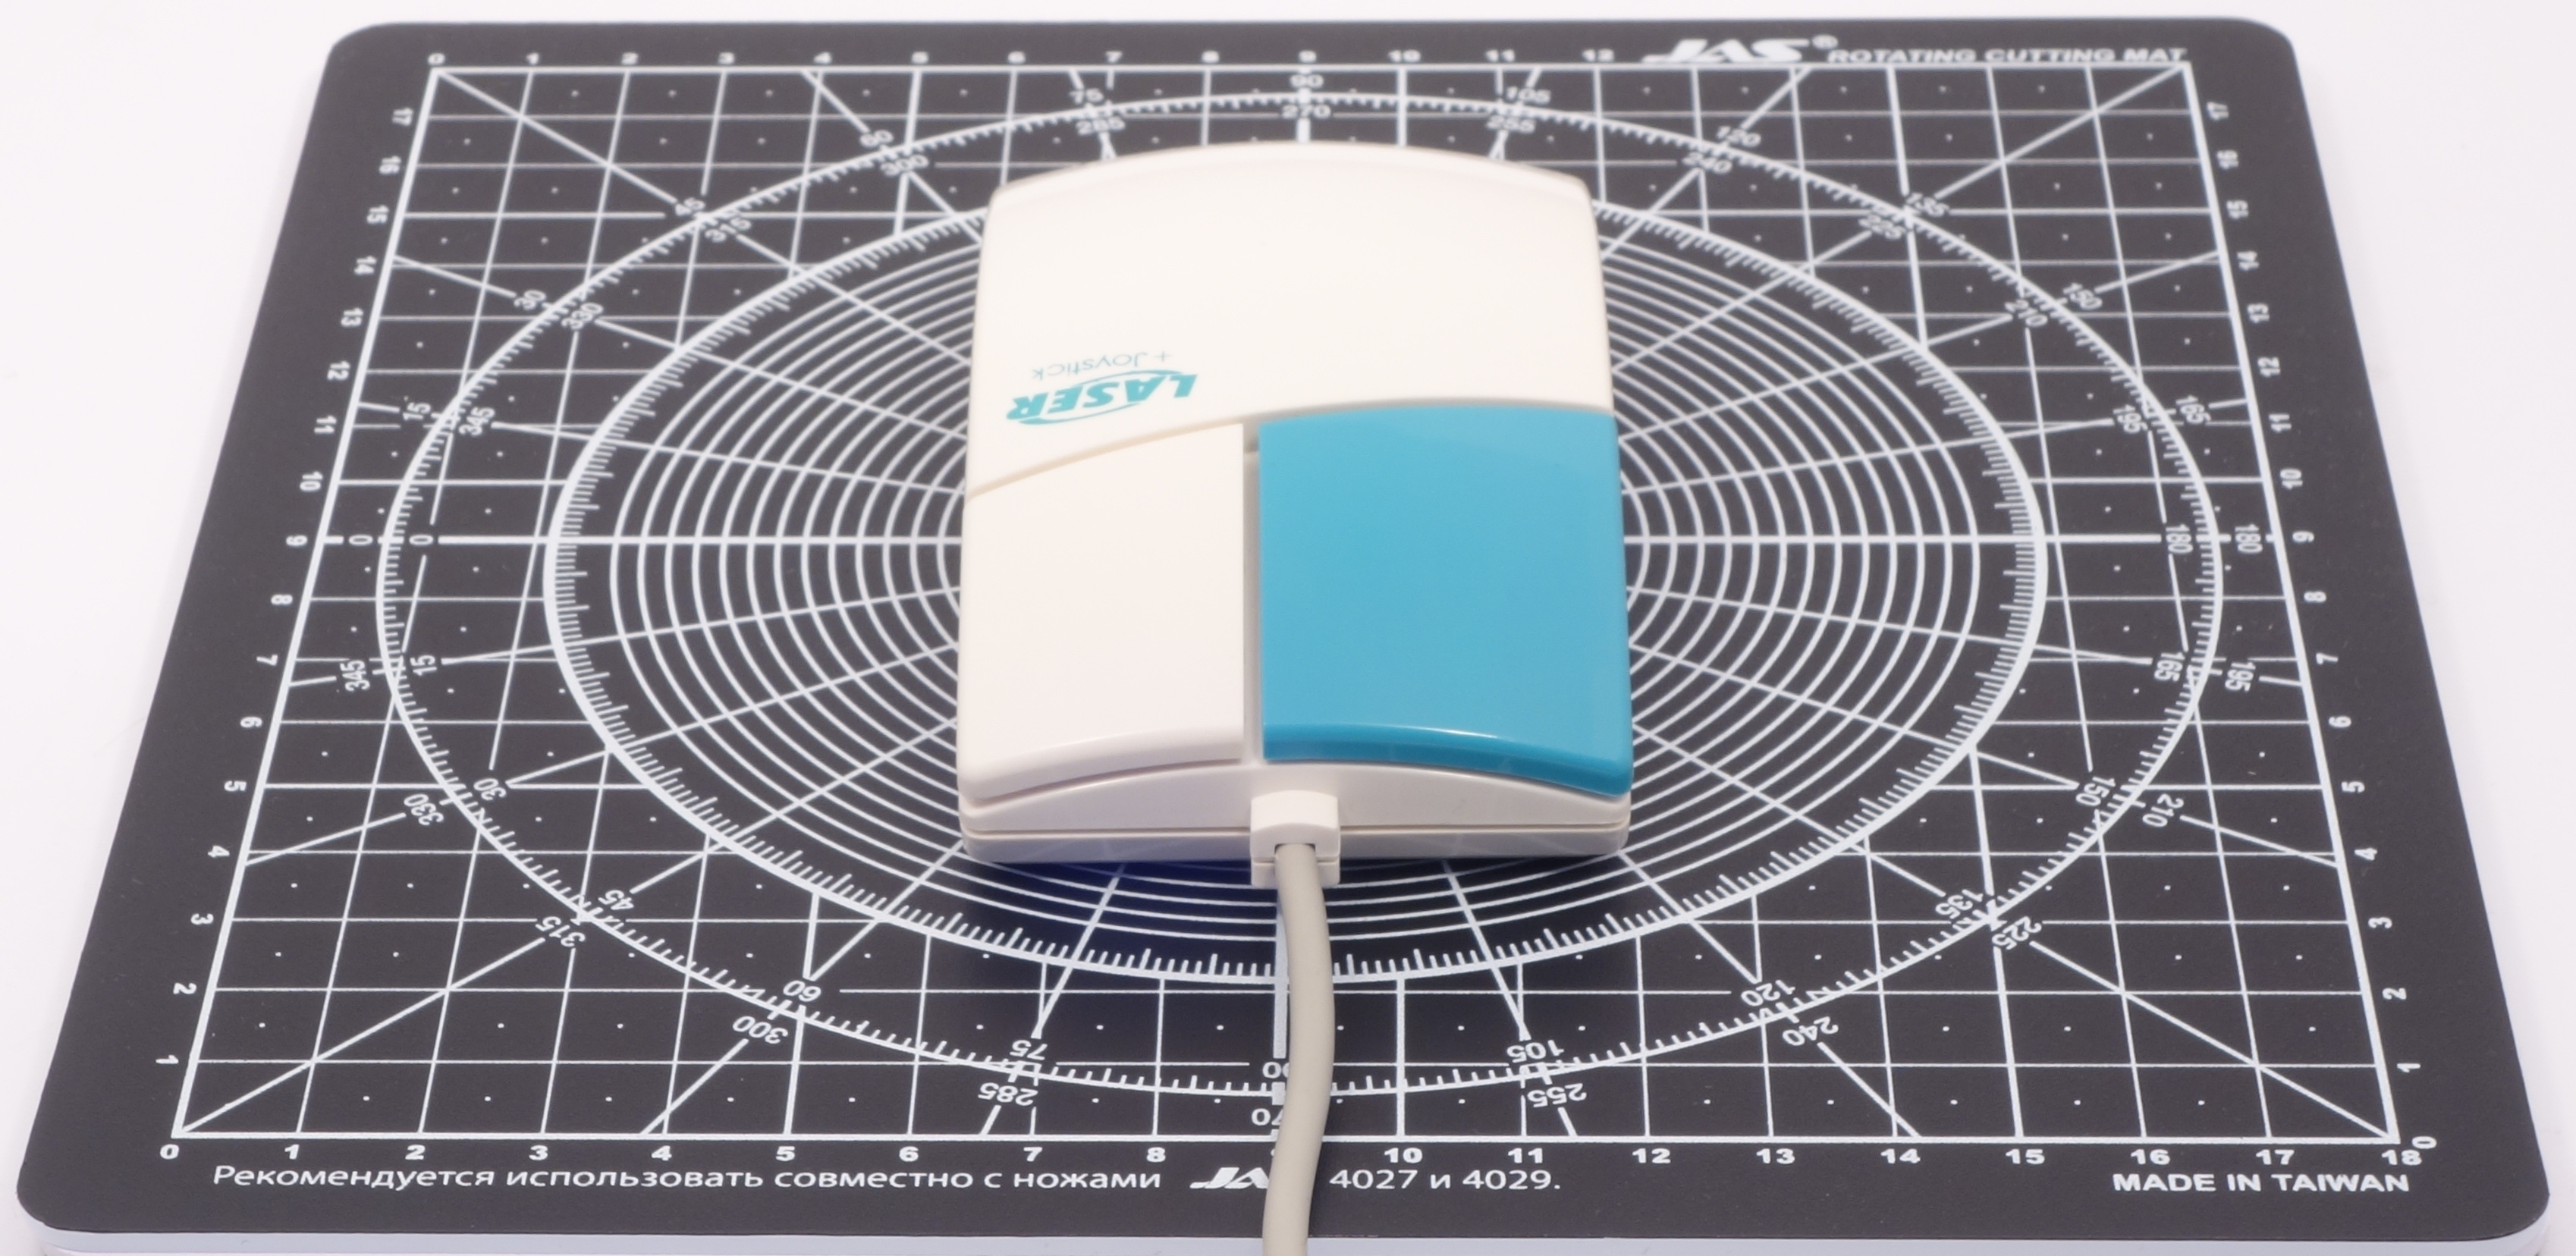
\includegraphics[scale=0.3]{1996_hi-bon_laser_mouse/size.jpg}
    \caption{Hi-Bon Optical laser mouse on a graduated pad with a grid step of 1~cm}
    \label{fig:OpticalLaserMouseSize}
\end{figure}

The third button, quite conveniently located on the side of the body in the reach of the thumb (figure \ref{fig:OpticalLaserMouseHand}) is used to switch modes. Additionally, this side button emulates a double press, but given its small area (unlike the main two), this function is not very convenient for frequent use.

\begin{figure}[h]
    \centering
    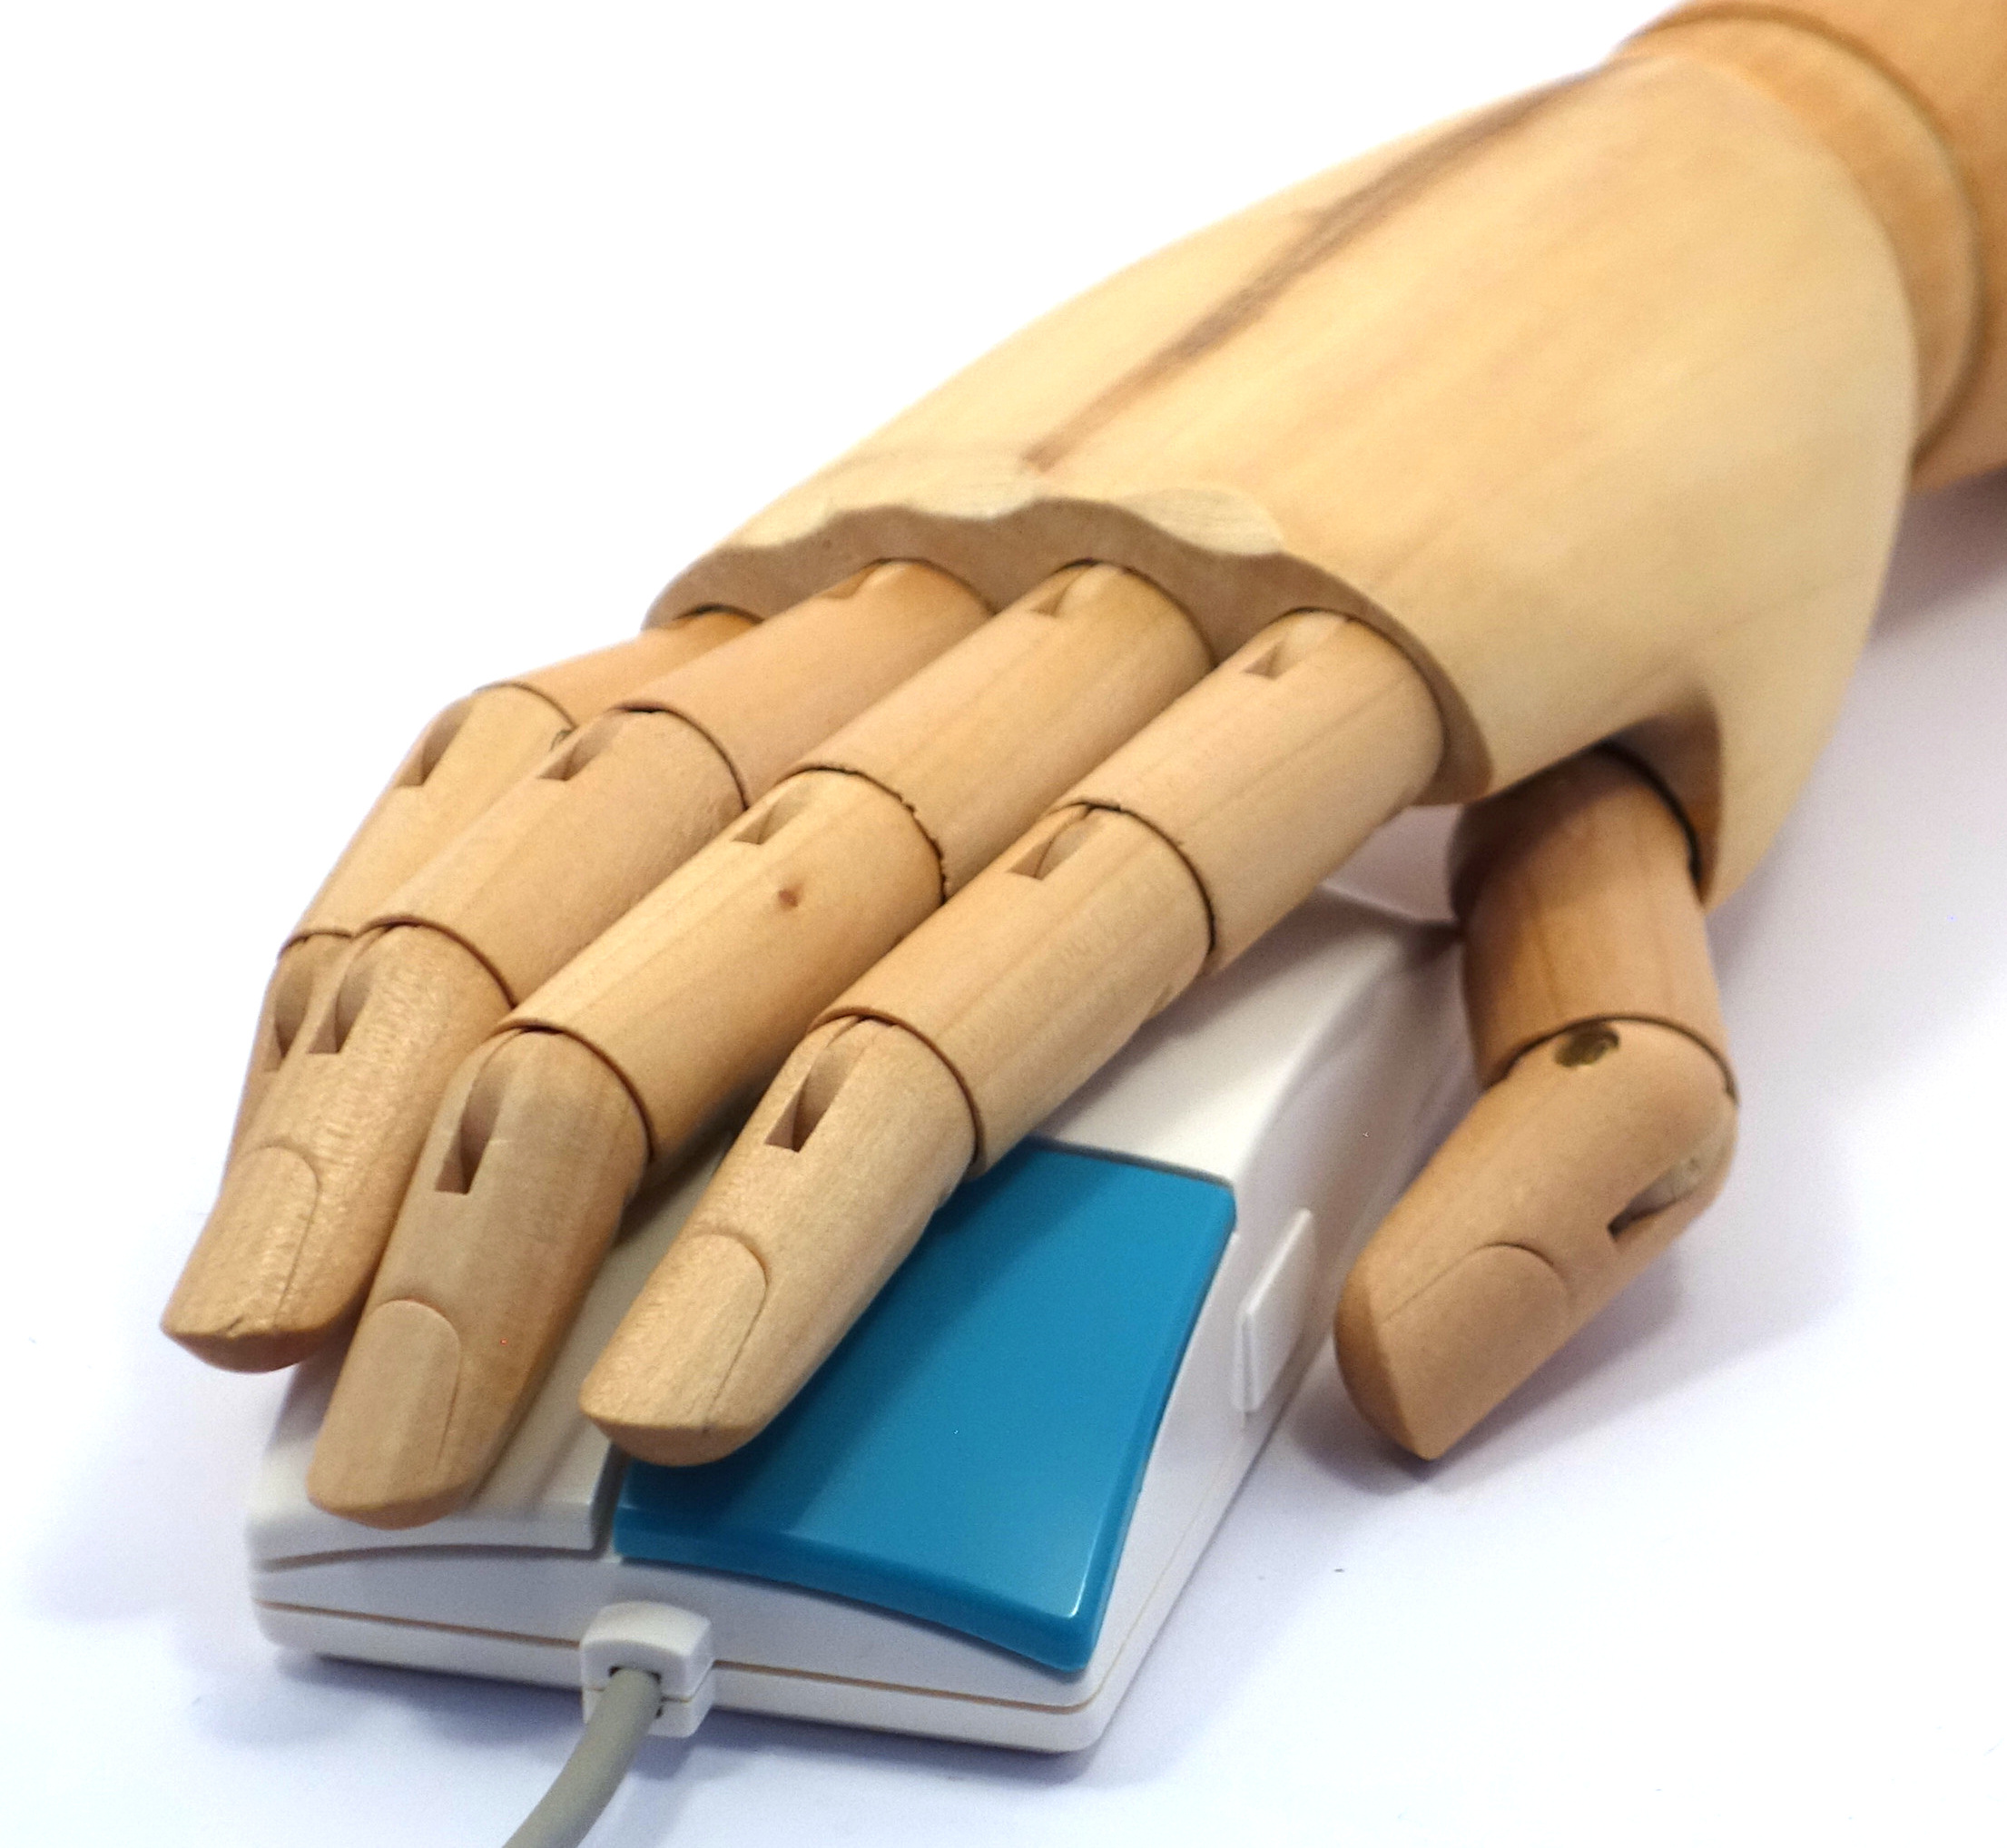
\includegraphics[scale=0.3]{1996_hi-bon_laser_mouse/hand_60.jpg}
    \caption{Hi-Bon Optical laser mouse with a human hand model}
    \label{fig:OpticalLaserMouseHand}
\end{figure}

Laser mouse contains a microcontroller that implements 3 modes of operation.

The first mode is standard. The second one (turned on by simultaneously pressing an additional button on the side of the case and the left mouse button) switches the mouse to joystick mode. In this mode, moving the mouse away from the center (the point at which the mouse was at the moment the mode was switched) is interpreted as a movement of the stick. It should be noted that using the mouse as a joystick is quite inconvenient in games \cite{LittleMagick}, given that the center to which you need to return to stop the character's movement is not marked in any way.

The third mode (turned on by simultaneously pressing the side and right buttons) activates the so-called “precision” mode, designed for artists and designers (in fact, it activates the declared resolution of 450 DPI).

Mouse internals are shown on figure \ref{fig:OpticalLaserMouseInside}). Two beams of light fibers go to four photo receivers. The use of a double number of photo receivers allowed the developers not to use the pad with longitudinal and transverse stripes (unlike a cheaper Q500 model and optical Mouse Systems mice), but use a grid of dark points instead. Thanks to this, turning the pad at $90^\circ$ does not affect the performance of the mouse. However, angles which are not multiple of 90 make it difficult to read the movement, and the $45^\circ$ angle makes it almost impossible to control the cursor\cite{comparison}.

\begin{figure}[h]
    \centering
    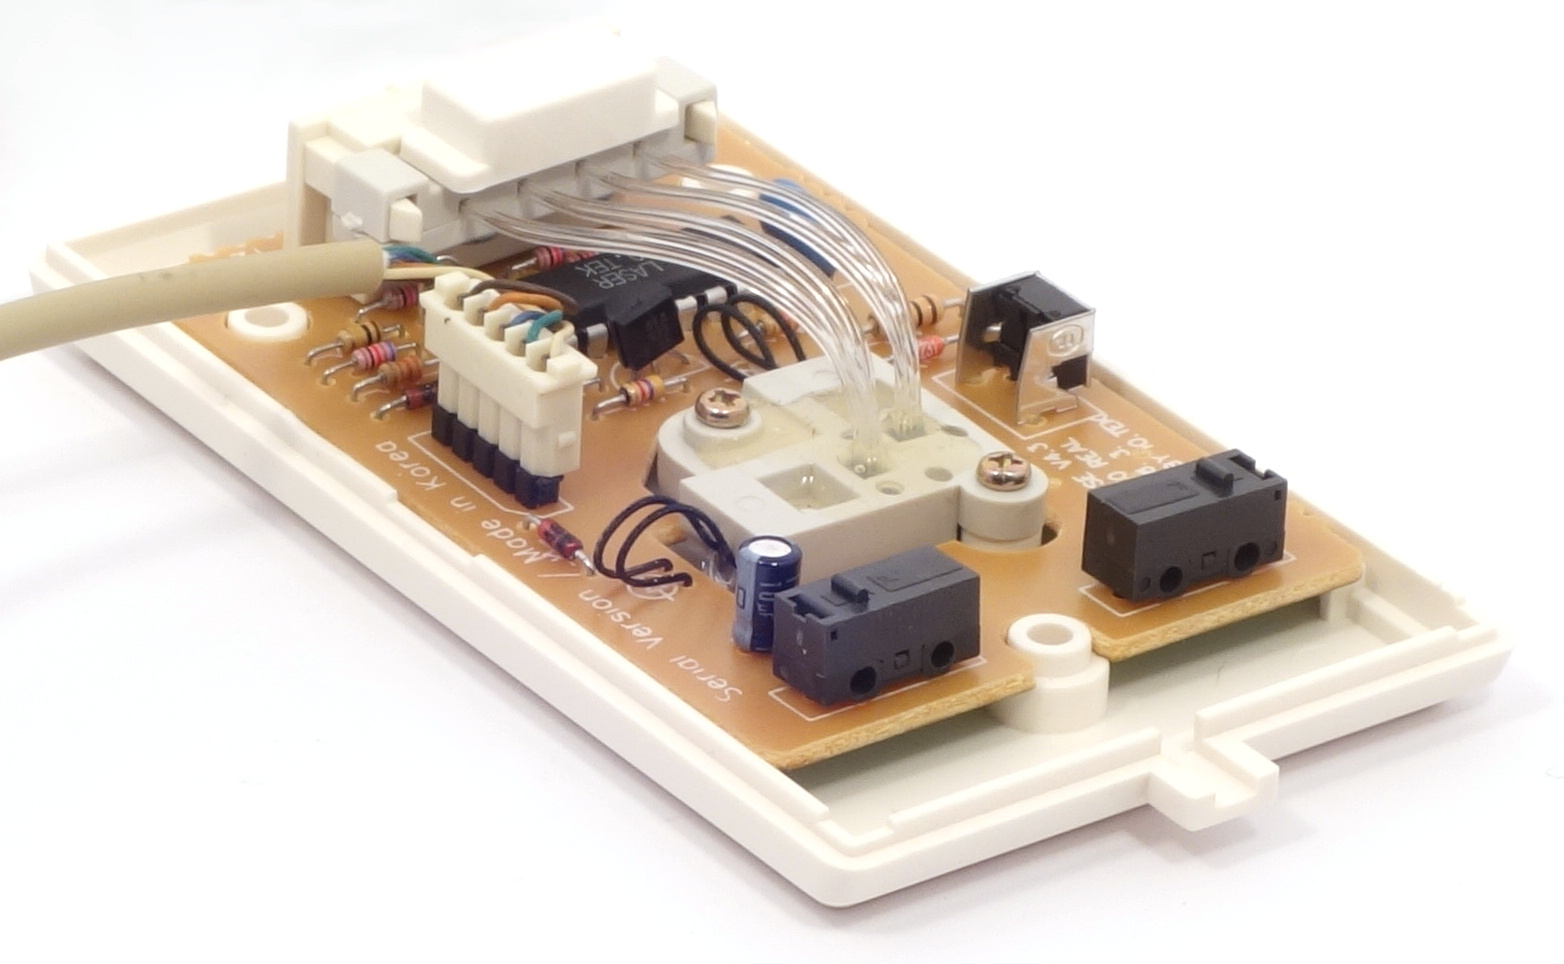
\includegraphics[scale=0.8]{1996_hi-bon_laser_mouse/inside_60.jpg}
    \caption{Hi-Bon Optical laser mouse disassembled}
    \label{fig:OpticalLaserMouseInside}
\end{figure}

The text on the PCB shows that this mouse was, like the Q500 mouse, developed under contract by iO TEK in 1996.

\begin{thebibliography}{9}
\bibitem{LittleMagick} This Serial ''Optical Laser Mouse'' from 1996 \url{https://www.youtube.com/watch?v=8CeKiSn5lGU}
\bibitem{comparison} LMOX2, The Other Weirdest Mouse \url{https://www.youtube.com/watch?v=2UXmDuiqMW0}

\end{thebibliography}
\end{document}
